\chapter{Reproducible and open library}
\label{chap:peerannot}
\enlargethispage{3\baselineskip}

\begin{keypointstwomargins}{Reproducible and open library}{-2cm}{-1cm}
        \textbf{Key points -- Community based data but what about codes\dots}
        \begin{enumerate}[leftmargin=*]
        \item Reproducibility has been a demand from the scientific community. With crowdsourcing, the coupling of the label gathering step and the aggregation is key to create a classical supervised learning dataset. Different label aggregation strategies can lead to widely different results. Releasing publicly available datasets original version with collected labels would lead to better data quality.
        \item More than the data itself, as the crowdsourcing community is made of researchers with very diverse backgrounds, new models arise quickly. In multiple coding languages (if any) and with personalized data formats. We need formatting propositions that can handle large datasets, are easily accessible and understandable.
        \item Aggregation strategies are often EM-based with a two steps procedure repeated. While performance is an important decision factor in using one strategy over another, how much time they take to run is essential. Especially with large datasets, we find memory scaling issues or a time complexity that forbids usage in applications.
        \end{enumerate}

        \textbf{Contributions -- peerannot and BenchOpt}
        \begin{enumerate}[leftmargin=*,start=4]
        \item We propose a new Python library \texttt{peerannot} fully documented. An \texttt{identify} module lets users identify ambiguous tasks from datasets using a wide range of strategies. The \texttt{aggregate} module performs label aggregation strategies. The \texttt{aggregate-deep} module uses learning strategies that are deep-learning based and have inserted the aggregation step inside the network's architecture. The \texttt{train} module allows to train classifiers from aggregated labels. Our library comes with data templates and examples available at \url{http://peerannot.github.io}
        \item We created a crowdsourcing benchmark in the \texttt{BenchOpt} library to easily compare time performance on label aggregation strategies across libraries, on publicly available datasets.
        \end{enumerate}
\end{keypointstwomargins}

\section{\texttt{peerannot}: Open access for crowdsourcing strategies in python}

The experiments ran in \Cref{chap:waum} made us realize key points in the field of crowdsourcing. The first one is that the data is often not released in a format that is easily usable -- when released. The second is that most of the time, the code is not released -- or partially released without functions and easy access to run new experiments, or also scattered with each their different programming language (python, R, stan, java,\dots). The third is that existing libraries to handle crowdsourcing data lack implemented strategies to identify poorly performing workers and/or ambiguous tasks.
Thus, we created the \texttt{peerannot} library.

Crowdsourced datasets induce at least three major challenges to which we contribute with \texttt{peerannot}:

\begin{enumerate}
  \item \textbf{How to aggregate multiple labels into a single label from crowdsourced tasks?} This occurs, for example, when dealing with a single dataset that has been labeled by multiple workers with disagreements. This is also encountered with other scoring issues such as polls, reviews, peer-grading, \textit{etc.} In our framework, this is treated with the \texttt{aggregate} command, which given multiple labels, infers a label. From aggregated labels, a classifier can then be trained using the \texttt{train} command.
  \item \textbf{How to learn a classifier from crowdsourced datasets?} Where the first question is bound by aggregating multiple labels into a single one, this considers the case where we do not need a single label to train on, but instead train a classifier on the crowdsourced data, with the motivation to perform well on a testing set. This end-to-end vision is common in machine learning; however, it requires the actual tasks (the images, texts, videos, \textit{etc.}) to train on -- and in crowdsourced datasets publicly available, they are not always available. This is treated with the \texttt{aggregate-deep} command that runs strategies where the aggregation has been transformed into a deep learning optimization problem.
  \item \textbf{How to identify good workers in the crowd and difficult tasks?} When multiple answers are given to a single task, looking for who to trust for which type of task becomes necessary to estimate the labels or later train a model with as few noise sources as possible. The module \texttt{identify} uses different scoring metrics to create a worker and/or task evaluation.
\end{enumerate}

The library \texttt{peerannot} addresses these practical questions within a reproducible setting and an easy-to-follow pipeline presented in \Cref{fig:pipeline_crowdsourcing_peerannot}. Indeed, the complexity of experiments often leads to a lack of transparency and reproducible results for simulations and real datasets.
We propose standard simulation settings with explicit implementation parameters that can be shared.
For real datasets, \texttt{peerannot} is compatible with standard neural network architectures from the \texttt{Torchvision} \citep{torchvision} library and \texttt{Pytorch} \citep{pytorch}, allowing a flexible framework with easy-to-share scripts to reproduce experiments.

\begin{figure}[ht]
        \centering
        \includegraphics[width=\textwidth]{chapters/images/strategies_crowd_data.pdf}
        \caption{Pipeline on how to handle crowdsourced datasets with \texttt{peerannot}. After collecting the data, the \texttt{identify} module helps find poorly performing workers and/or ambiguous tasks. Those can be pruned to recover a \emph{cleaned} set. Then, the \texttt{aggregate} module can be used to infer a label from multiple labels. The \texttt{aggregate-deep} module can be used to train a classifier from the crowdsourced labels without aggregation. Finally, the \texttt{train} module can be used to train a classifier from aggregated labels.}
        \label{fig:pipeline_crowdsourcing_peerannot}
    \end{figure}

\subsection{Identification, aggregation and learning}

The \texttt{peerannot} library is available on \url{https://peerannot.github.io/} and can be installed using \texttt{pip}:
\begin{minted}[linenos=true, bgcolor=lightgray, tabsize=4, fontfamily=courier, fontsize=\small, xleftmargin=5pt, xrightmargin=5pt]{bash}
$ pip install peerannot
\end{minted}

When installed, it comes with both a \texttt{python} Application Programming Interface (API) and a Command Line Interface (CLI).
Note that the \texttt{python} API is the main interface to use the library, and the CLI is a wrapper around the \texttt{python} API to make it easier to use for non-programmers.
Moreover, the CLI can be used in a \texttt{python} program in interactive cells using the \texttt{!} character to run the shell commands indicated by the dollar sign \texttt{\$}.

\subsubsection{Dataset standardization}

Crowdsourced datasets come in various forms. To store crowdsourcing datasets efficiently and in a standardized way, \texttt{peerannot} proposes the following structure, where each dataset corresponds to a folder. Let us set up a toy dataset example to understand the data structure and how to store it.

\begin{figure}[htb]
        \centering
\begin{forest}
        for tree={
            font=\ttfamily,
            grow'=0,
        %     child anchor=west,
        %     parent anchor=south,
        %     anchor=west,
            folder indent=.9em, folder icons,
        edge=densely dotted,
        % sep=10pt,
                       }
        [datasetname
            [ $\ \text{train}$
                [$\ \text{...}$]
                [$\ \text{images}$]
                [$\ \text{...}$]
            ]
            [$\ \text{val}$]
            [$\ \text{test}$]
            [metadata.json, is file]
            [answers.json, is file]
        ]
\end{forest}
\end{figure}

The \texttt{answers.json} file stores the different votes for each task as described in \Cref{fig:json}. This \texttt{.json} is the rosetta stone between the task IDs and the images. It contains the tasks’ id, the workers’s id and the proposed label for each given vote. Furthermore, storing labels in a dictionary is more memory-friendly than having an array of size $(n_{task}, n_{worker})$ and writing $y_i^{(j)}=-1$ when the worker $w_j$ did not see the task $x_i$ and $y_i^{(j)}\in[K]$ otherwise.

\begin{figure}[htb]
\centering
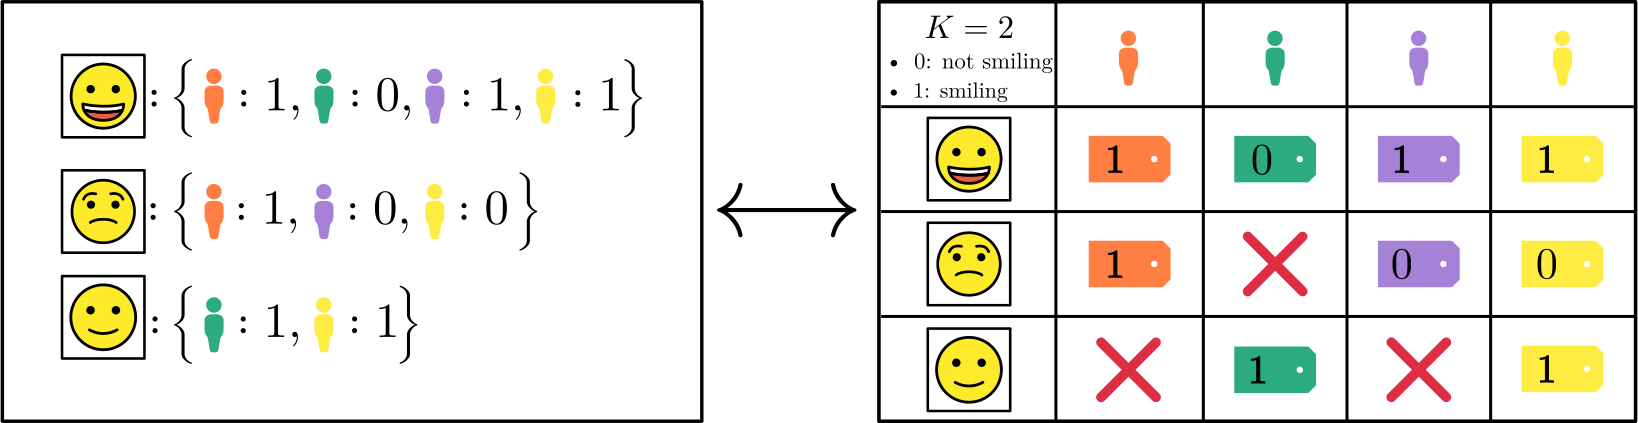
\includegraphics[width=\textwidth]{./images/json_answers.pdf}
\caption{Data storage for the \texttt{toy-data} crowdsourced dataset, a binary classification problem ($K=2$, smiling/not smiling) on recognizing smiling emoticons. On the left how \texttt{peerannot} stores the data, and on the right the raw data.}
\label{fig:toy-data}
\end{figure}

Finally, a \texttt{metadata.json} file includes relevant information related to the crowdsourcing experiment such as the number of workers, the number of tasks, \emph{etc.} For example, a minimal \texttt{metadata.json} file for the toy dataset presented in \Cref{fig:toy-data} is:
\begin{minted}[linenos=true, bgcolor=lightgray, tabsize=4, fontfamily=courier, fontsize=\small, xleftmargin=5pt, xrightmargin=5pt]{json}
{
    "name": "toy-data",
    "n_classes": 2,
    "n_workers": 4,
    "n_tasks": 3
}
\end{minted}


The toy-data example dataset is available as an example in the \texttt{peerannot} repository. Classical datasets in crowdsourcing such as \texttt{CIFAR-10H} \citep{peterson_human_2019} and \texttt{LabelMe} \citep{rodrigues2014gaussian} can be installed directly using \texttt{peerannot}. To install them, run the \texttt{install} command from \texttt{peerannot}:

\begin{minted}[linenos=true, bgcolor=lightgray, tabsize=4, fontfamily=courier, fontsize=\small, xleftmargin=5pt, xrightmargin=5pt]{bash}
$ peerannot install ./datasets/labelme/labelme.py
$ peerannot install ./datasets/cifar10H/cifar10h.py
\end{minted}

For both \texttt{CIFAR-10H} and \texttt{LabelMe}, the dataset was originally released for standard supervised learning (classification). Both datasets have been reannotated by a crowd of workers.

\subsubsection{Other popular formats}

Other popular storage formats currently exist.
For example, the \texttt{crowd-kit} \citep{CrowdKit2023} uses a dataframe where each row specifies the $3$-uplet $($task, worker, label$)$.
This format is close to the \texttt{json} one, easily switchable between the two. However, it suffers from the redundancy of the task ID.

The \texttt{LabelMe} dataset labels are stored in a dense matrix of size $(n_{\text{task}}, n_{\text{worker}})$, where each entry is the label given by the worker for the task. This format is not memory efficient for a large number of tasks or workers. Especially if workers do not get to label all tasks.

On a more practical note, the \texttt{json} format has the advantage of being easily readable and writable by humans and is also easily convertible to a data frame. It is also easy to use for \texttt{python}, \texttt{SQL} and \texttt{JavaScript}.
As large crowdsourcing web platforms use requests in \texttt{JavaScript} to send and receive data, the \texttt{json} format is a motivating choice for applications.

\subsection{Label agggregation with \texttt{peerannot}}

In addition to the classical MV, NS, DS, GLAD aggregation strategies presented in \Cref{sub:aggregating_votes}, \texttt{peerannot} proposes a growing number of aggregation strategies to fit different needs.
The full list is available by running the command:

\begin{minted}[linenos=true, bgcolor=lightgray, tabsize=4, fontfamily=courier, fontsize=\small, xleftmargin=5pt, xrightmargin=5pt]{bash}
$ peerannot agginfo
\end{minted}


For example, the Worker Clustered DS model (DSWC) by \citet{imamura2018analysis} is based on the DS model.
Each worker belongs to one of the $L\leq n_{\text{worker}}$ clusters.
This strategy highly reduces the number of parameters.
In the original DS strategy, there are $K^2\times n_{\text{worker}}$ parameters to estimate for the confusion matrices. The DSWC strategy has $K^2\times L + L$ parameters to estimate.
Indeed, there are $L$ confusion matrices $\Lambda=\{\Lambda_1,\dots,\Lambda_L\}$ of size $K\times K$ and the confusion matrix of a cluster is assumed drawn from a multinomial distribution with weights $(\tau_1,\dots,\tau_L)\in\Delta_L$ over $\Lambda$ such that $\mathbb{P}(\pi^{(j)}=\Lambda_\ell)=\tau_\ell$ for $\ell \in [L]$.

\paragraph{Structure of a label aggregation strategy.}

All of the label aggregation strategies are stored in the \texttt{peerannot.models} module.
Each strategy is a class object in its own \texttt{python} file.
It inherits from the \texttt{CrowdModel} class template and is defined with at least three methods:
\begin{itemize}
    \item \texttt{run}(): includes the optimization procedure to obtain needed weights (\emph{e.g.} the EM algorithm for DS). It is only needed for optimization-based strategies.
    \item \texttt{get\_probas}(): returns the soft labels output for each task after running the \texttt{run} method,
    \item \texttt{get\_answers}(): returns the hard labels output for each task after running the \texttt{run} method.
\end{itemize}

\paragraph{Example of a label aggregation strategy.}

For example, let us consider minimal working examples (MWE) for the \texttt{NS} and the \texttt{DS} strategies.
The first in \Cref{listing:NS} is a non-parametric strategy without any optimization algorithm, and the second in \Cref{listing:DS} is an EM-based parametric strategy.

\begin{listing}[!ht]
\begin{minted}[linenos=true, bgcolor=lightgray, tabsize=4, fontfamily=courier, fontsize=\small, xleftmargin=5pt, xrightmargin=5pt]{python}
from ..template import CrowdModel
import numpy as np


class NaiveSoft(CrowdModel):
    def __init__(self, answers, n_classes=2, **kwargs):
        super().__init__(answers)
        self.n_classes = n_classes

    def get_probas(self):
        baseline = np.zeros((len(self.answers), self.n_classes))
        for task_id in list(self.answers.keys()):
            task = self.answers[task_id]
            for vote in list(task.values()):
                baseline[task_id, vote] += 1
        self.baseline = baseline
        return baseline / baseline.sum(axis=1).reshape(-1, 1)

    def get_answers(self):
        return np.vectorize(self.converter.inv_labels.get)(
            np.argmax(self.get_probas(), axis=1)
        )
\end{minted}
\caption{MWE for the NS label aggregation in \texttt{peerannot}.}
\label{listing:NS}
\end{listing}


\begin{listing}[!ht]
    \begin{minted}[linenos=true, bgcolor=lightgray, tabsize=4, fontfamily=courier, fontsize=\small, xleftmargin=5pt, xrightmargin=5pt]{python}
class Dawid_Skene(CrowdModel):
    def __init__(self, answers, n_classes, **kwargs):
        super().__init__(answers)
        self.n_classes = n_classes
        self.n_workers = kwargs["n_workers"]
        self.n_task = len(self.answers)

    def get_crowd_matrix(self):
        ... # Convert json answers to tensor (task, worker, label)

    def init_T(self):
        ... # Initialize the confusion matrices

    def m_step(self):
        """Maximizing log likelihood
        Returns:
            p: (p_j)_j class marginals
            pi: confusion matrices
        """
        ...

    def e_step(self):
        """Estimate indicator variables
        Returns:
            T: New estimate for the labels (n_task, n_worker)
        """
        ...

    def log_likelihood(self):
        ... # Compute the log likelihood of the model

    def run(self, epsilon=1e-6, maxiter=50):
        self.get_crowd_matrix()
        self.init_T()
        k, eps, ll = 0, np.inf, []
        while k < maxiter and eps > epsilon:
            self.m_step()
            self.e_step()
            likeli = self.log_likelihood()
            ll.append(likeli)
            if len(ll) >= 2:
                eps = np.abs(ll[-1] - ll[-2])
            k += 1

    def get_probas(self):
        return self.T

    def get_answers(self):
        return np.vectorize(self.converter.inv_labels.get)(
            np.argmax(self.get_probas(), axis=1)
        )
\end{minted}
\caption{MWE for the DS label aggregation in \texttt{peerannot}.}
\label{listing:DS}
\end{listing}

If a new user wants to add their strategy, they can follow the same structure and add it to the \texttt{peerannot} library. The strategy will then be available for all users to use through a pull request.

\section{Benchmarking aggregation strategies with \texttt{Benchopt}}
XXX with Axel
\subsection{What is \texttt{Benchopt}?}
XXX take back the article a bit

\subsection{Results with crowdsourcing real datasets}
XXX Panoplie de datasets let's go sur les aggregations